\subsection{Position changing}
\label{sec:position_change}

To simulate the presence of multiple vehicles a list of fake coordinates can be dinamically assigned to each device during a simulation. Figure \ref{fig:positions} shows an example of how positions are dinamically assigned in the application we built for Android devices in order to implement a testbase application for the Fast Broadcast algorithm (an analogous method is used in Desktop version).

Let's suppose we have four devices, namely A, B, C and D, and suppose we have eight different positions. At the beginning, we have A, B, C and D assigned rispectively to positions 1, 2, 3 and 4. At a certain moment device A broadcasts an \emph{Alert message}. As soon as the messages is sent, device A is assigned to position 5. The other devices compute the \textit{Contention Window} and wait for a random time in the intervall $[0,Contention Window]$ before retransmitting the \emph{Alert}. In figure \ref{fig:positions} devices \textit{Contention Window} is represented as a yellow right triangle, this because it decreases with the increase of the distance from the source. Now let's assume that device C forwards the message because its timeout expires for first: as required by the algorithm, devices B and D will detect the transmission from C and abort the retransmission of A's message. In order to carry on with the simulation, device B (which received C's message from behind) moves from position 2 to position 6, and then reconsider C's message for retransmission. This process continues until the last available position is reached.
In both implementations the starting positions are assigned as soon as the initial setup is completed. In the Android application, the designated \textit{group owner} assigns a progressive number to each device, which represents the line in the position file from which the device should read the first position. Supposing $N$ devices are involved in the simulation, when a device needs to switch position, it will simply skip $N-1$ lines after the current one.
With this iterative mechanism we can distribute a certain number of virtual devices on a route of arbitrary lenght. 
We also use distance filters to simulate real devices range: every time a message is received, the distance from the sender and the receiver is computed and, if it is greater than the (configurable) maximum wireless range, it is discarded.
Position reassignment policy and message filtering based on wireless range, have to be specified in each protocol implementation, and can be achieved generating the corrisponding events.

\begin{figure}[htbp]
\centering
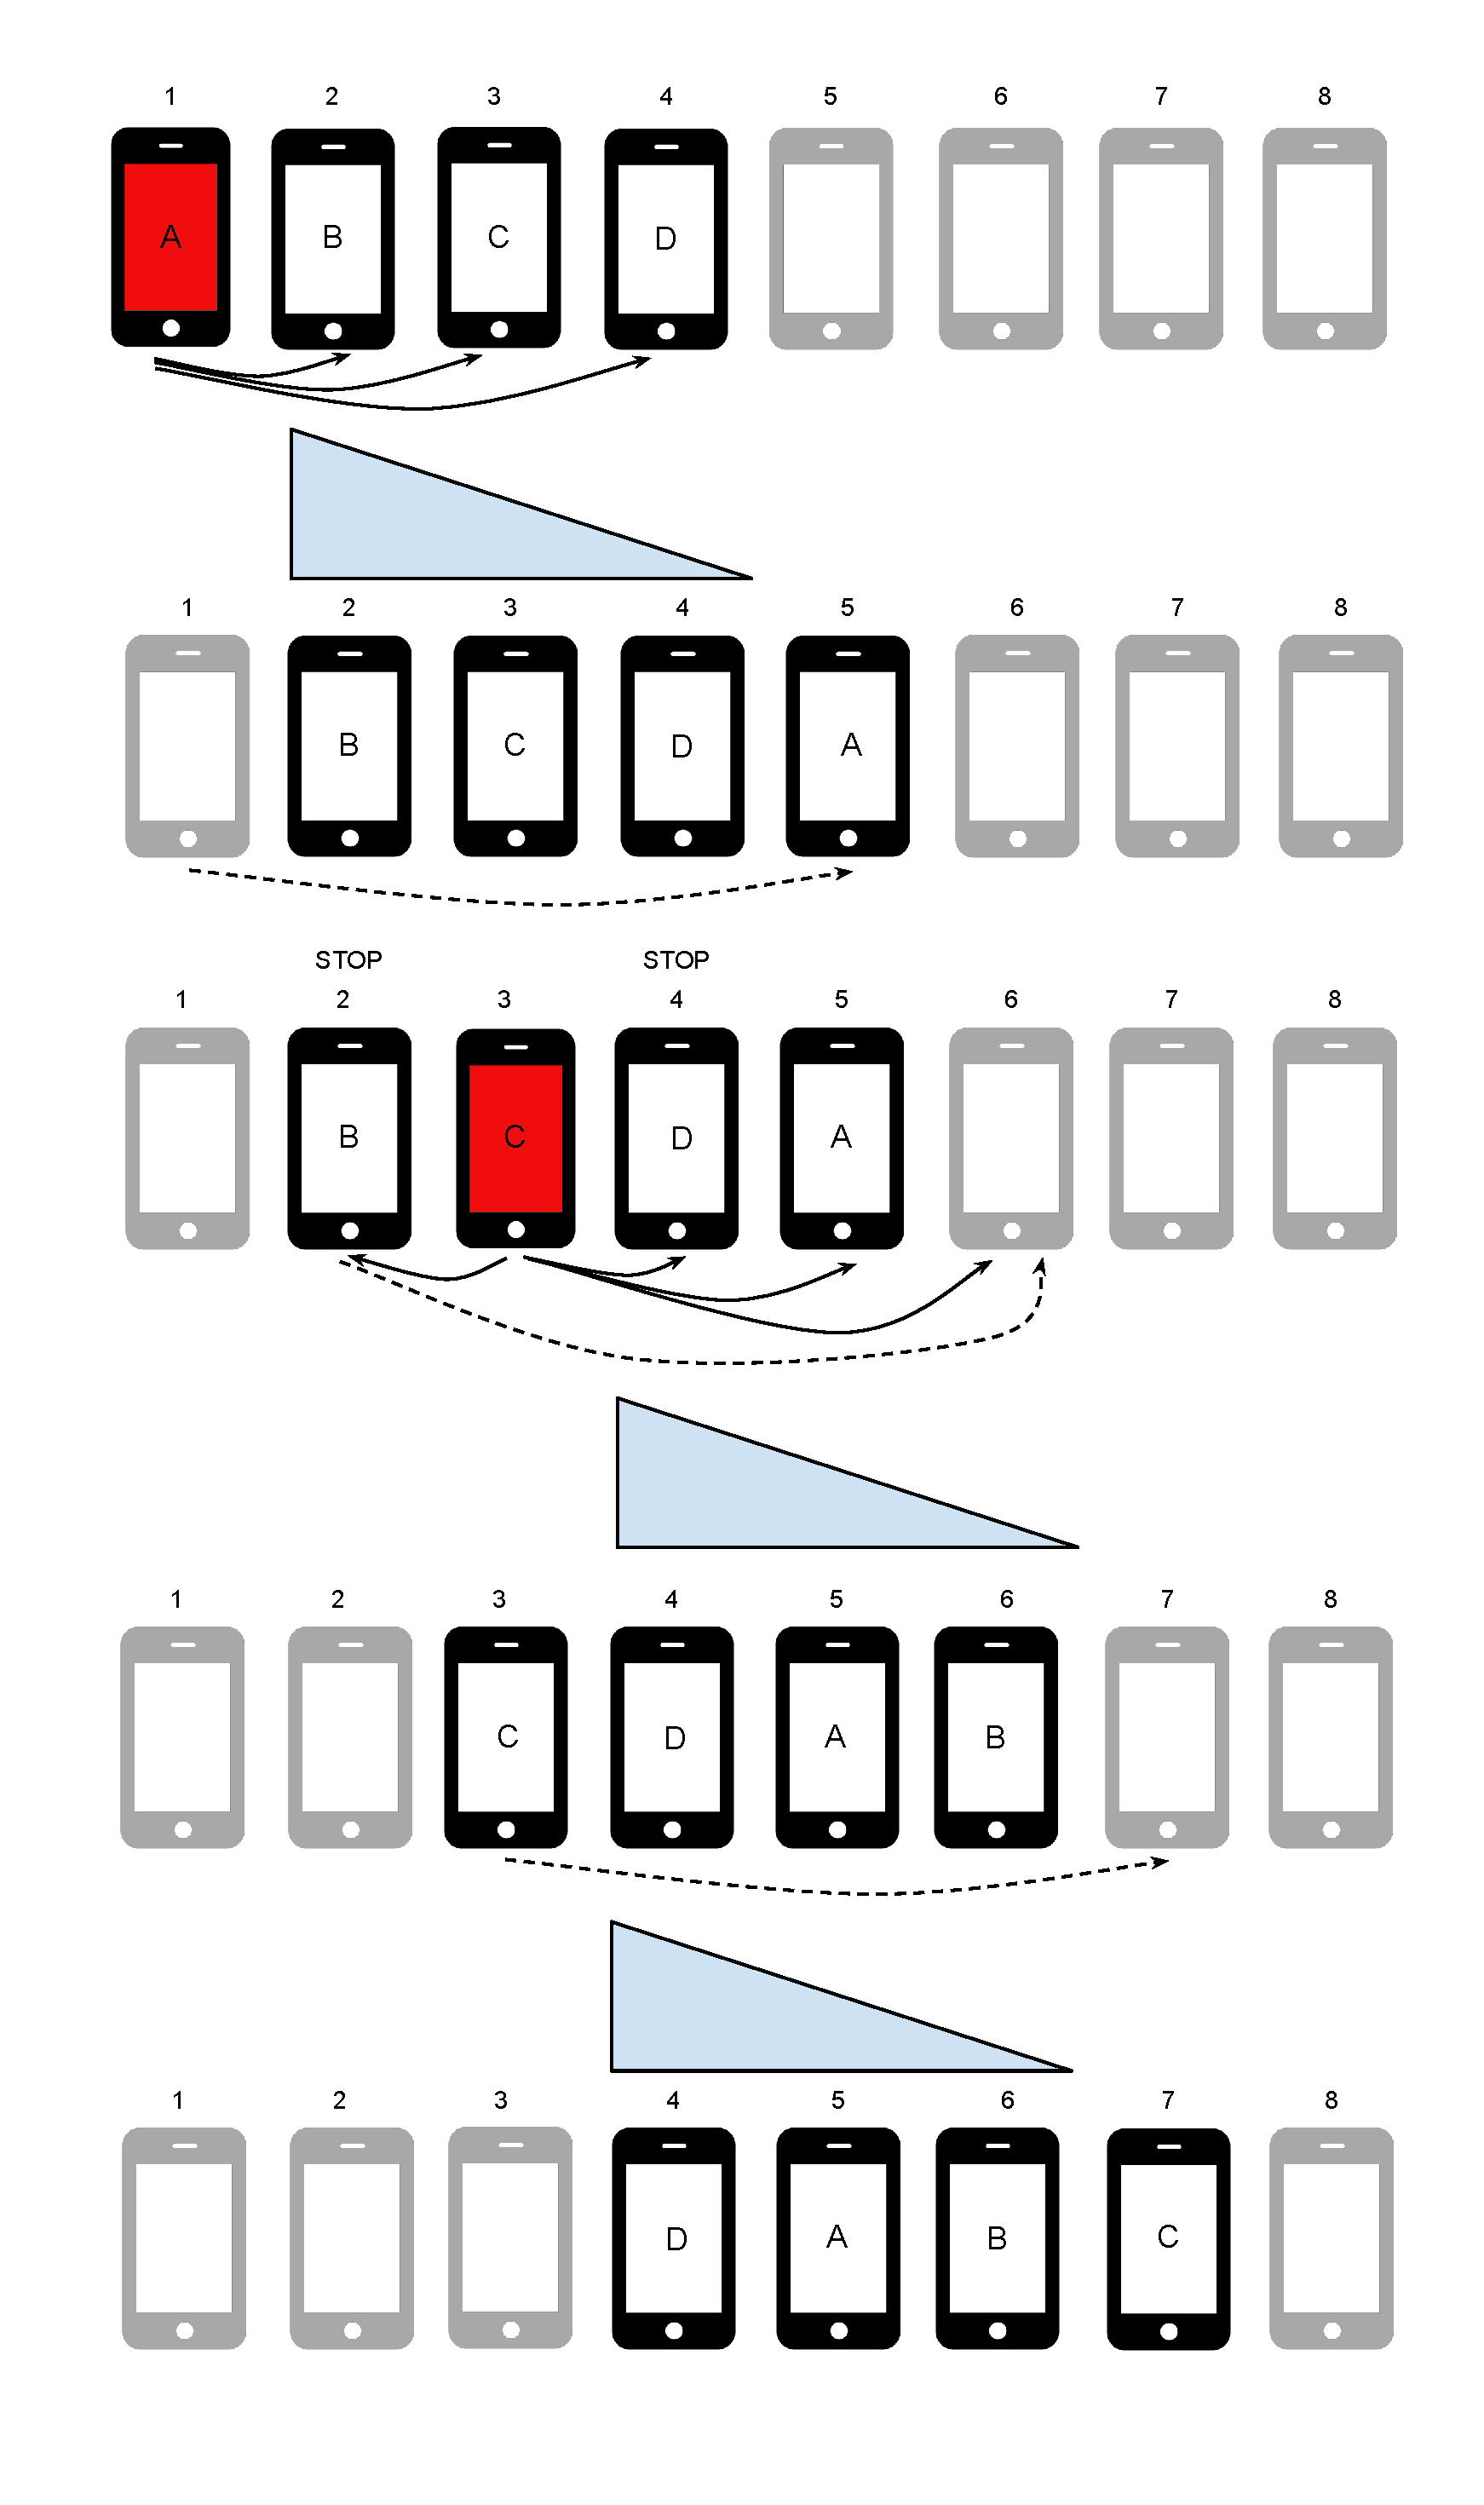
\includegraphics[trim = 10mm 15mm 10mm 10mm ,width=3.5in]{imgs/Positions_1.pdf}
\caption{Devieces position changes}
\label{fig:positions}
\end{figure}
